\chapter{CubeSat Design}

	Für die Realisierung einer ADR-Mission liegt der Fokus zunächst bei dem Entwurf eines geeigneten CubeSats. Infolgedessen wird in diesem Kapitel ein bestehendes Konzept \cite{Lettau.} anhand der Software QuSAD (SQL-Based CubeSat Analyse and Design Tool QuSAD) analysiert und gegebenenfalls optimiert. Zuvor wird ein Einblick in das Programm gegeben und durch eine anschließende Beschreibung des angenommenen Entwurfs erfolgt abschließend die Budgetplanung. Letztlich wird mittels der Budgets eine Auswertung des Designs bezüglich seiner Effizienz durchgeführt. Bei Bedarf werden Verbesserungen in Erwägung gezogen. Demnach kann ein zielführendes Missionsdesign bestimmt und bewertet werden.
		
		\section{QuSAD}
			
			\subsection{Einführung in die Software}
			
	
	Die Software QuSAD (SQL-Based CubeSat Analyse and Design Tool) besteht aus einem SQL-Segment und einem MatLab Segment. Die SQL-Datenbank ist die Haupteingabequelle für das Entwerfen eines CubeSats und kategorisiert die CubeSat-Komponenten. Durch die wissenschaftliche Version können die COTS-Komponenten mit vordefinierten Parametern eingepflegt werden. Des Weiteren können auch individuelle Komponenten mit veränderbaren Parametern mittels der praxis Version hinzugefügt werden. Für das Abrufen der Komponententabelle aus der SQL-Datenbank wird MatLab verwendet. Dies wird durch mehrere grafische Benutzeroberflächen (GUI) realisiert und ermöglicht dem Benutzer eigene Satellitenzusammenstellungen. Neben dem CubeSat Design können Budget Analysen von Masse, Volumen, Energie, Preis und Verlinkung durch zur Verfügung stehenden Werkzeuge erstellt werden, um folglich eine Optimierung des Entwurfs zu ermöglichen. Für ein vertieftes Verständnis der Software wird auf das QuSAD-Handbuch \cite{Farahvashi.2016} verwiesen. Das Anwendungsspektrum von QuSAD umfasst das erstellen eines Satelliten, sowie eine Bereitstellung einer Datenbank von Subsystemen für wissenschaftliche und auch lehrende Aspekte. Lehrende Aspekte umfassen den Einsatz der praktischen Version an Universitäten zur Unterstützung und Visualisierung. \cite{Farahvashi.2016b}
			
			\subsection{Datenbankerweiterung}
			
			Zur Erweiterung der Datenbank wird anfänglich die Auswahl der CubeSat-Komponenten einer ausgewählten Systemzusammenstellung verwendet (siehe \tab{tab:cubesatdesign}). Zu den besagten Komponenten werden alle bekannten Werte der Datenbank hinzugefügt. Des Weiteren müssen Recherchen bezüglich weiterer Herstellerangaben durchgeführt werden. Im Fokus liegen dabei alle Parameter die für die Budgetsplanungen benötigt werden. Angesichts der Budgetanalyse des zusammengestellten Satelliten wird eine Optimierung einiger COTS-Komponenten vorgenommen und dementsprechend die Datenbank um weitere Subsysteme erweitert. Zur Unterstützung der Ergänzungen wird eine interne Datenbank genutzt. Diese wurde von Mitarbeitern des Institutes Raumfahrtsysteme der Technischen Universität Braunschweig erstellt. Überwiegend sind die aufgelisteten Systeme mit einem TRL Wert hinterlegt. Da in vielen Fällen nur erprobte Systeme zum Einsatz kommen, werden Komponenten mit einem TRL Wert von 9 mit in die Datenbank hinzugefügt. Zusätzlich sind Internet-Quellenverweise (URL - Uniform Resource Locator) zu den meisten Einträgen vorhanden, über die man häufig direkt oder indirekt auf Datenblätter weitergeleitet wird und an weitere Informationen bezüglich des Subsystems gelangt.
			%\subsection{Problematiken}
			%Die Datenbankerweiterung und Budgeterstellung führte zu einigen Schwierigkeiten. Bei dem Laden der Datenbank über den SQL Server traten Fehlermeldungen bei MatLab auf, die nicht behoben werden konnten. Die Ursache könnte an der Inkompatibilität zwischen den neuen MatLab Versionen und MySQL liegen, da QuSAD mit der MatLab Version R2014 erstellt wurde. Im QuSAD Handbuch wird auf dieses Problem hingewiesen. Infolgedessen wurde die Datenbank über MySQL importiert und Lokal darauf zugegriffen. Die Datenbank wird in Mat-File Dateien gespeichert und kann über MatLab aufgerufen werden. Anschließend können die Komponenten in die gespeicherte Datenbank eingepflegt und als Workspace gesichert werden. Durch das Exportieren der neuen Datenbank über MySQL wird der Zugriff künftig bereitgestellt. Besonders problematisch gestaltete sich das einpflegen der Komponenten in die Datenbank. Im Handbuch, sowie den weiteren Dokumenten zur Datenbank wurde der Vorgang nicht hinreichend genau beschrieben. Des Weiteren gab es viele unbekannte Angaben über die hinzugefügten Komponenten. Diese mussten einzeln recherchiert und in seltenen fällen abgeschätzt werden. In der bereitgestellten Datenbank vom Institut fehlten an wichtigen Daten für die Budgets in den meisten fällen nur die Preise. Außerdem wurde festgestellt, dass einige URLs nicht mehr Gültig sind.
		
		\section{CubeSat Designanalyse}
				
				\subsection{Angenommenes Design}
				
				Die CubeSat Konfiguration orientiert sich an einem entwickelten Design \cite{Lettau.}. Hier wurde ein ausführlicher Vergleich und anschließend eine Auswertung der in betracht gezogenen Subsysteme durchgeführt. Im Folgenden wird auf die ausgewählten Komponenten eingegangen um einen Überblick über die darauf folgenden Budgets zu gewähren. Bei der Beschreibung werden die Komponenten in die folgenden Kategorien: 
				\begin{itemize}
					\item Antenne
					\item Antrieb
					\item Batterie
					\item Kontroll Bord
					\item EPS
					\item Nutzlast und Verschiedenes 
					\item Solar Panele
					\item Tracker und Sensors
					\item Transceiver
					\item Struktur
				\end{itemize}
eingeordnet. Dies orientiert sich an der Struktur der QuSAD Datenbank. In der \tab{tab:cubesatdesign} sind alle Komponenten in der entsprechenden Kategorie und der Mengenangabe aufgelistet. Zusätzlich befindet sich im \anh{tab:} die \tab{tab:} mit allen relevanten Werten der einzelnen Komponenten auf die in diesem Kapitel eingegangen wird.
				\begin{table}[!h]
				\centering
\begin{tabular}{|l|l|c|}
\hline
\multicolumn{1}{|c|}{Subsystem} & \multicolumn{1}{c|}{Produkt}    	            & Anzahl \\ \hline
Antenne                         & IQW S-Band Dual Patch Antenna                 & 2      \\ \hline
                                & SkyFox Labs piPATCH-MAX (GNSS)                & 2      \\ \hline
Kontroll Board                  & SSTL OBC750 LEO Flight Computer               & 1      \\ \hline
EPS                             & NanoAvionics EPS                              & 1      \\ \hline
Nutzlast \& Verschiedenes       & Vision-based LiDAR Sensor                     & 1      \\ \hline
                                & Crystalspace CAM1U 5 MP (RNS)                 & 2      \\ \hline
                                & Gecko based                                   & 1      \\ \hline
Antrieb                         & Iodine tank                                   & 1      \\ \hline
                                & Nitrogen tank                                 & 1      \\ \hline
                                & Busek BHT-200 Thruster (electric)             & 1      \\ \hline
                                & Marotta Micro-Thruster (chemical)             & 24     \\ \hline
Solar Panel                     & Top/Bottom BCT 9U                             & 1      \\ \hline
                                & BCT 9U Tripple Wing Solar Array Custom (Side) & 1      \\ \hline
                                & BCT SADA Gimbal System                        & 1      \\ \hline
Transceiver                     & IQW Slink-Phy S-Band Transceiver              & 1      \\ \hline
Struktur                        & 27U NanoAvionics Standard Structure (s)       & 1      \\ \hline
Tracker \& Sensor               & TY-Space PST3                                 & 2      \\ \hline
                                & NSS Fine Sun Sensor NFSS-411                  & 4      \\ \hline
                                & Sensonor STIM300                              & 1      \\ \hline
                                & SSTL SGR-Ligo                                 & 1      \\ \hline
\end{tabular}
\caption{Angenommenes Design \cite{Lettau.}}
\label{tab:cubesatdesign}
\end{table}

	Vorweg wird auf die betrachteten Anforderungen, die beim Entwicklungsprozess entscheidend  sind, eingegangen. Die Konzeptplanung knüpft an der SpaceX-Starlink-Konstellation an. Davon abgeleitet wird für die Umlaufbahnparamter und die Raumfahrzeugeigenschaften von folgenden Parametern ausgegangen. Es wird der, für die Mission ungünstigste Fall betrachtet der bei einem Neigungswinkel von 0$\textdegree$ und einer Missionsdauer von 10 Jahren liegt (siehe \tab{tab:parameter}).
\begin{table}[!h]
\centering
	\begin{tabular}{|l|c|c|}
\hline
\multicolumn{1}{|l|}{Parameter}          & \multicolumn{1}{l|}{Starlink} & \multicolumn{1}{l|}{Verwendete} \\ \hline
\multicolumn{1}{|l|}{Höhe {[}km{]}}      & \multicolumn{1}{c|}{1150}     & \multicolumn{1}{c|}{1150}       \\ \hline
\multicolumn{1}{|l|}{Neigung {[}\textdegree{]}} & \multicolumn{1}{c|}{53}       & \multicolumn{1}{c|}{58}       \\ \hline
\multicolumn{1}{|l|}{Sonnenwinkel {[}\textdegree{]}}       & \multicolumn{1}{c|}{-}        & \multicolumn{1}{c|}{0}          \\ \hline
\multicolumn{1}{|l|}{Zeit {[}Missionsdauer {Jahr]}}      & \multicolumn{1}{c|}{1150}     & \multicolumn{1}{c|}{1150}       \\ \hline
          
	\end{tabular}
	\caption{Eigenschaften des ausgewählten Raumfahrzeug Starlink und die verwendeten Parameter \cite{Lettau.}}
	\label{tab:parameter}
\end{table}

	
	Als Primärstruktur ist ein 27U CubeSat mit einer zugelassen maximalen Masse von 50 kg und eine Gesamtabmessung von 34 x 35 x 36 cm verwendet (siehe \abb{fig:27U}). 				
				\begin{figure}[!h]
					\centering
						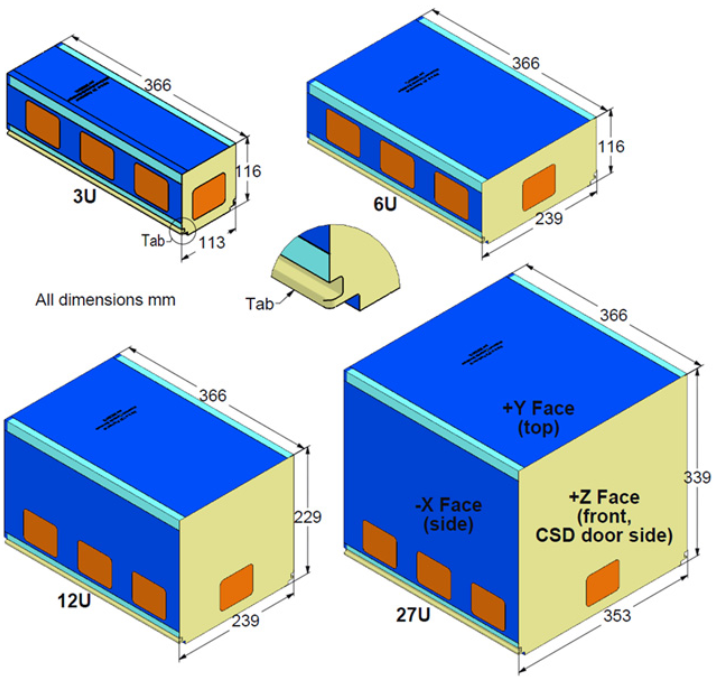
\includegraphics[width=0.60\textwidth]{27U}
					\caption{CubeSat-Größen gemäß der Planetary Systems Corporation \cite{Lettau.}}
					\label{fig:27U}
				\end{figure}

	Das Hauptantriebssystem ist der BHT-200 und wird mit dem Treibstoff Iod betrieben. Hier handelt es sich um einen elektrischen Antrieb mit einem TRL-Wert von 8 und einem guten leistungspezifischen Schub von 65 $P_{sT} {\mu N}{W}$. Durch das geringe Volumen von 3 U und der Verwendung von leichten Materialen für die Tankwände bewährt sich Jod als Treibstoff. Bei der Annahme eines Neigungswinkels von 58 \textdegree ergibt sich beim BHT-200 eine Betriebsdauert von 16,1 \%. Als weiteres Triebwerk wird das chemische Triebwerk Marotta verwendet. Dies dient zur Ausführung von Manövern während des Anfahrens als auch für die Demontage und Stabilisierung beim Deorbiten mit hohen Stapelmassen. Durch die Auslegung der Kaltgaspakete für sehr kleine Satelliten (< 6U) weisen sie sehr geringe Schübe auf und erreichen nicht die 0,23 $N$. Desto Trotz werden 24 Marotta Triebwerke verwendet, um eine 6-DoF-Manövrierfähigkeit zu ermöglichen. Sie weisen im Vergleich zu anderen Kaltgastriebwerken einen hohen $I_{sp}$ Wert auf (siehe \tab{tab:Marotta}). Eine Anordnung der 24 Marotta Triebwerken befindet sich in der \abb{fig:marotta}. Dieses Triebwerk wird mit Stickstoff betrieben und benötigt zuzüglich von 40 \% Sicherheit und der Annahme einer Stabilisierung von einer Sekunde alle 10 Orbits  eine Gesamttreibstoffmasse von 2,12 $kg$.
\begin{figure}[!h]
\centering
	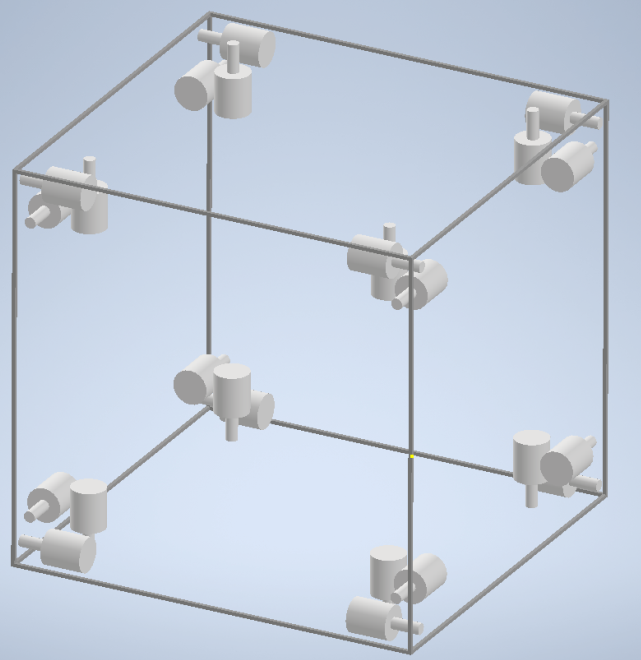
\includegraphics[width=0.30\textwidth]{Marotta}
	\caption{Anordnung der RCS-Triebwerke \cite{Lettau.}}
	\label{fig:marotta}
\end{figure}

	Viele Unternehmen bieten kundenspezifische Lösungen an. Dies wird auch von dem Unternehmen Blue Canyon Technologies für das Solarmodul 6U-H triple deployable solar array angeboten. Da es sich um eine zweiflügelige Konfiguration mit einer Grundfläche von 6U pro Flügel handelt, wird sie auf eine Grundfläche von 9U hoch skaliert damit sie auf  den 27U CubeSat angewendet werden kann. Des Weiteren wird von einer dreiflügeligen Konstellation ausgegangen. Die Vergrößerung der Solaranlage sorgt für eine Steigerung der Nennleistung um 50 \%. Weiterhin wird ein Solarpanel auf die obere Grundfläche des CubeSats platziert. Mit allen sieben Solarpanelen erreicht der CubeSat eine Nennleistung von 202 W. In der \abb{fig:solarpanel} ist eine vereinfachte CAD Darstellung von der Solaranlage. 
\begin{figure}[!h]
\centering
	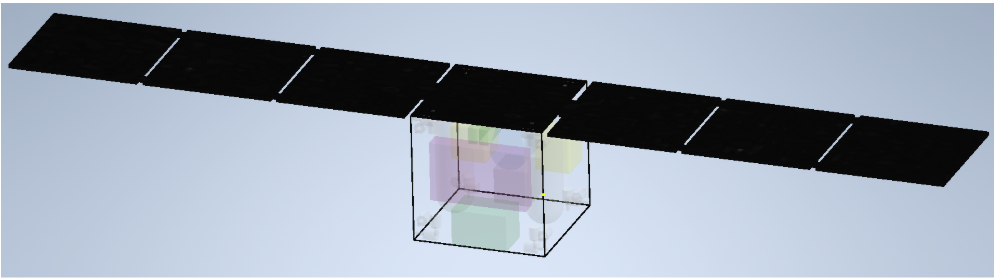
\includegraphics[width=0.60\textwidth]{graphics/Solarpanel.PNG}
	\caption{CAD Darstellung von der Solarkonfiguration \cite{Lettau.}}
	\label{fig:solarpanel}
\end{figure}

	Bei dem Power Management and Distribution System (PMAD-System) ist das NanoAvionics EPS, mit einem TRL von 9, dass geeignetste PMAD-System. Bei dieser Variante ist das besondere, dass ein externes Batteriepack mitgeliefert wird. Die EPS Variante kann eine Leistung von 175 W und eine Kapazität von 161 Wh liefern. Des Weiteren kann die Batterie skaliert werden um die Leistungsabgabe zu erhöhen.

						%Hier die Varainte von Max nehmen und kurz beschreiben
				\subsection{Budgetplanung}
Im folgenden Kapitel wird auf die mittels QuSAD erstellten Budgets für Masse, Volumen und Leistung eingegangen. In QuSAD werden Komponenten in Kategorien eingeteilt. Die Budgets werden mit diesen Kategorien erstellt. Eine Tabelle mit allen Kategorien und den dazugehörigen Komponenten ist im Kapitel 3.2 zu finden [Tabelle Kap. 3.2]

Die Batterie ist im EPS Board integriert und taucht darum im Massen- und Volumenbudget nicht auf. Da QuSAD in der Kategorie EPS keinen Eintrag über speicherbare Energie zulässt, wurde die Batterie nur für das Leistungsbudget hinzugefügt. Des weiteren ist zu beachten, dass die Komponenten in den unterschiedlichen Budgets keine einheitliche Farbgebung aufweisen. Einbauvorrichtungen wurden in QuSAD nicht bereücksichtigt. Die Abweichungen in den Budgets durch das  zusätzliche Gewicht und Volumen sind davon abhängig inwiefern die Herstellerangaben den Einbau berücksichtigen.

						\subsubsection{Massenbudget}
Das Massenbudget \abb{fig:masse} zeigt die aktuelle Massenverteilung des Designs an. Die maximal verfügbare Masse ist über eine Angabe in der Strukturkomponente begrenzt. Diese beinhaltet einen Wert für die maximale Gesamtmasse. Die maximale Gesamtmasse des CubeSats wurde mit 50 kg angenommen. Das aktuelle Design beansprucht circa 57 \% der möglichen Gesamtmasse (28,5 kg). Den größten Teil macht dabei die Antriebsanlage aus. Es gilt zu beachten, dass dieses Budget die Startmasse des CubeSats widerspiegelt. Nach Beginn der Mission ändert sich die Massenverteilung aufgrund des Treibstoffverbrauchs.
										\begin{figure}[!h]
											\centering
												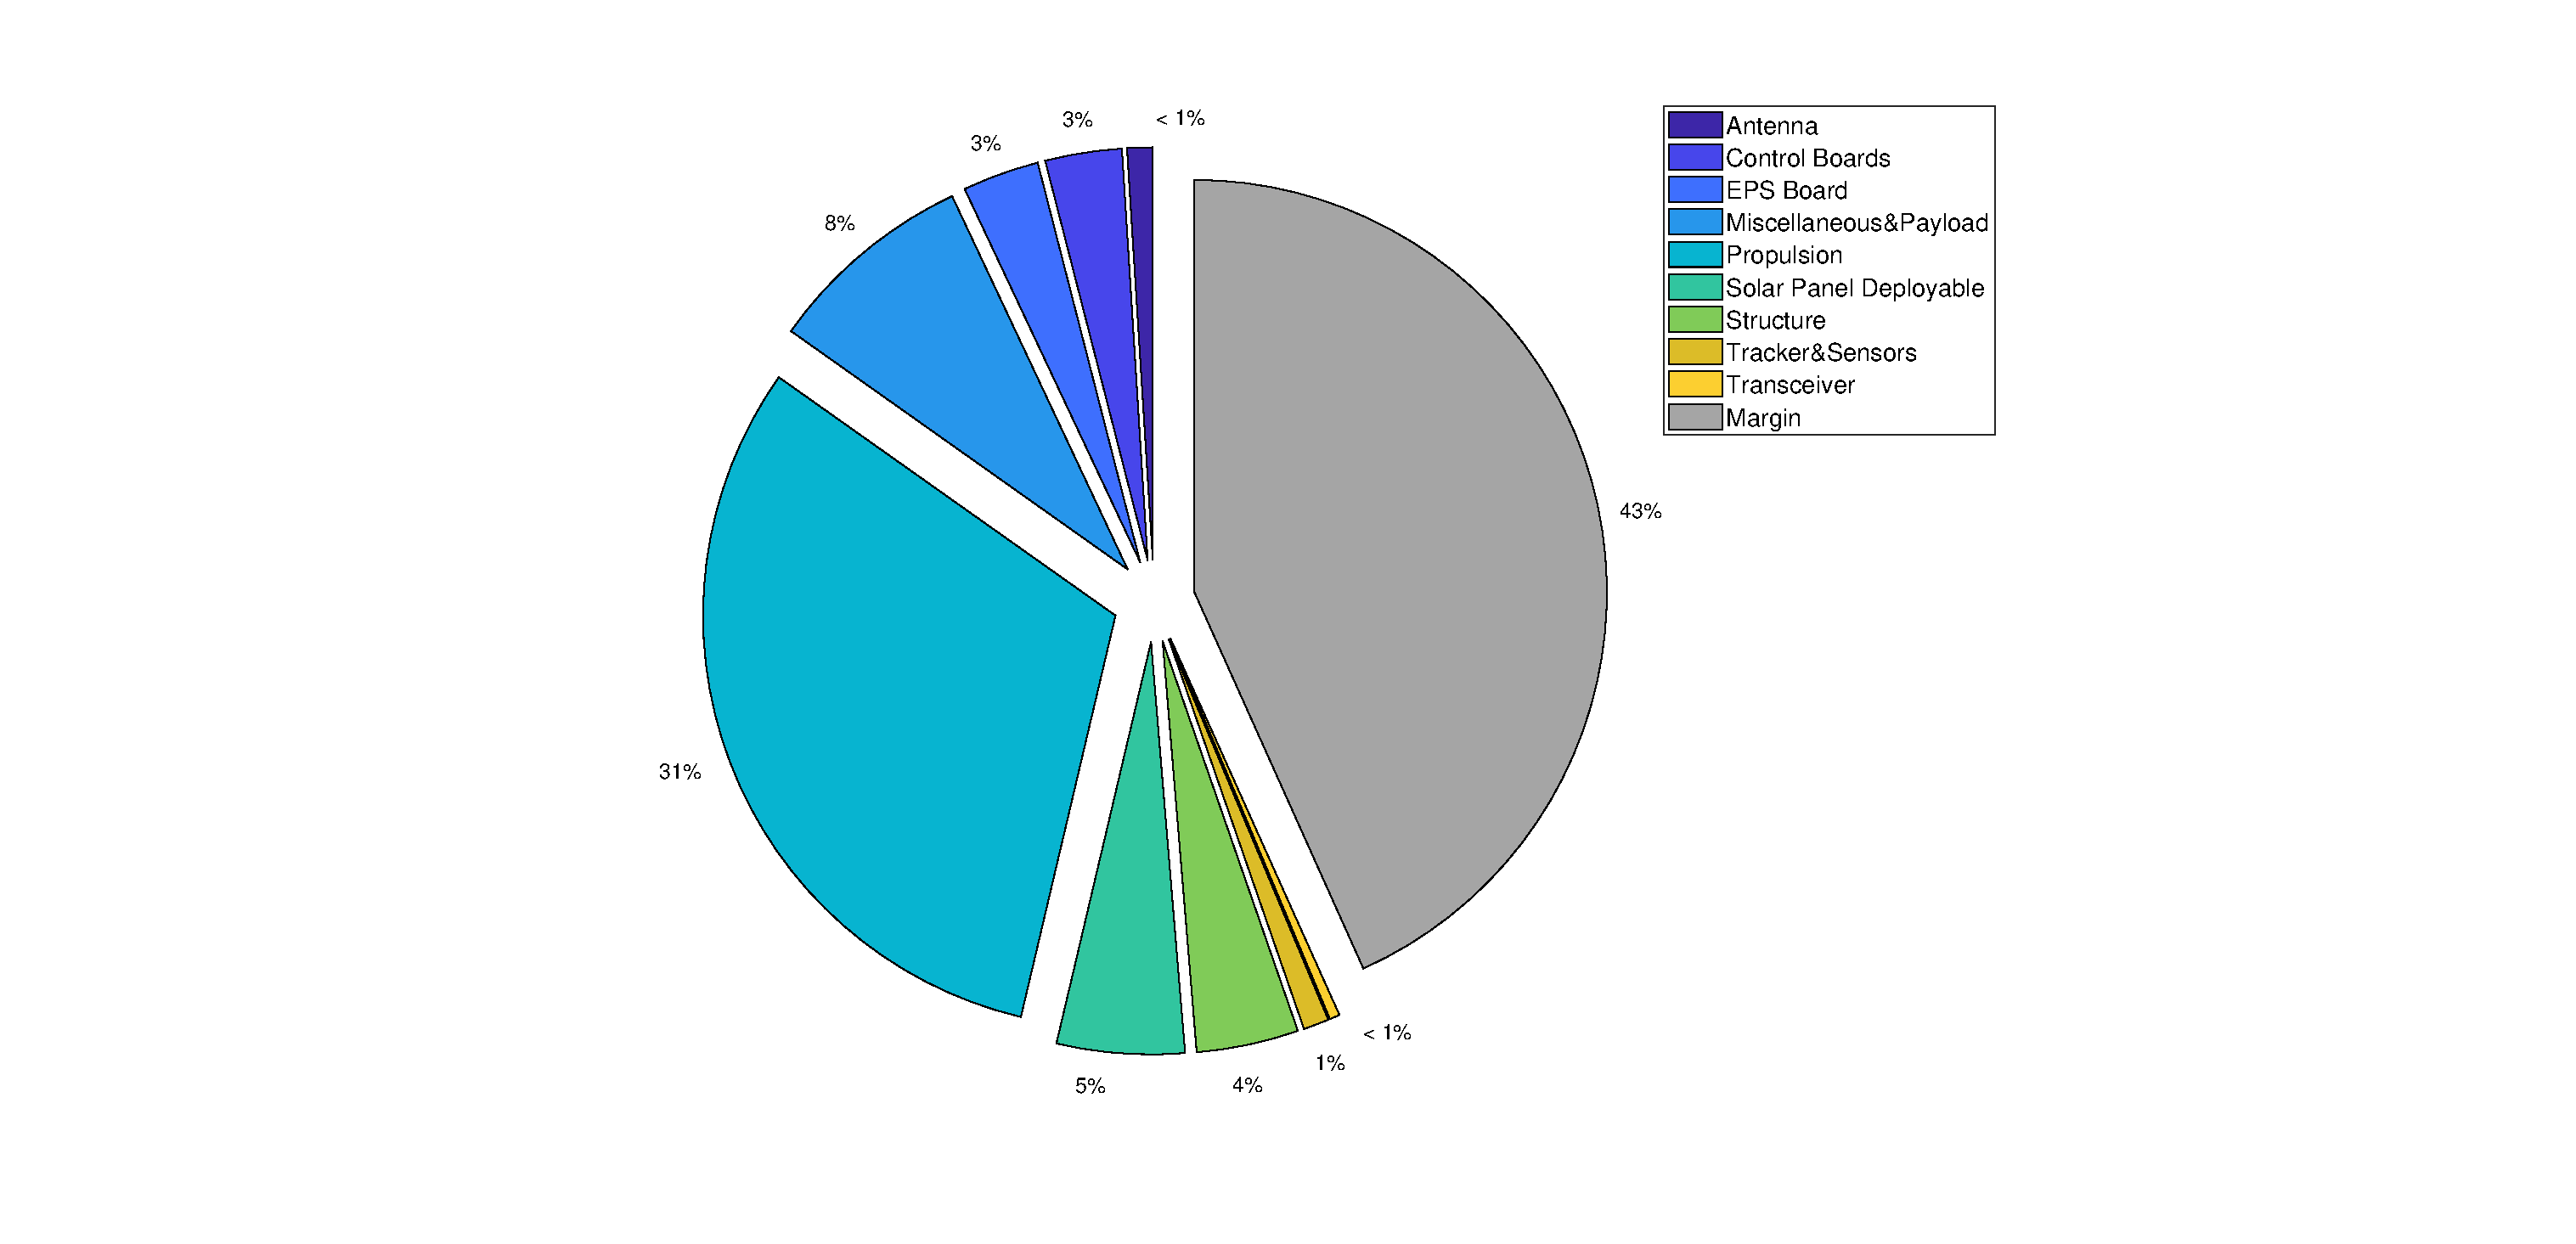
\includegraphics[width=0.90\textwidth]{masse}
											\caption{Massenbudget für das angenommene Design}
											\label{fig:masse}
										\end{figure}
										
						\subsubsection{Volumenbudget}
Das Volumenbudget \abb{fig:volume} gibt einen strukturierten Überblick über die aktuelle Volumenverteilung der ausgewählten Konfiguration, beziehungsweise des Profils in QuSAD. Das maximale verfügbare Volumen bemisst sich an der im Profil befindlichen Strukturkomponente, die über eine Volumenangabe verfügt. Das verfügbare Gesamtvolumen ist im Gegensatz zur Masse jedoch zu circa 97 \% ausgelastet. Es fällt auf, dass nahezu alle Kategorien einen größeren Volumenanteil als Massenanteil aufweisen. Das größte Volumen nimmt, ähnlich wie beim Massenbudget die Antriebsanlage ein. Sie macht jedoch aufgrund der Treibstofftanks über die Hälfte des Gesamtvolumens aus. Es sollte beachtet werden, dass aufgrund des geringen Freiraums kaum Sicherheiten möglich sind. 
								
										\begin{figure}[!h]
											\centering
												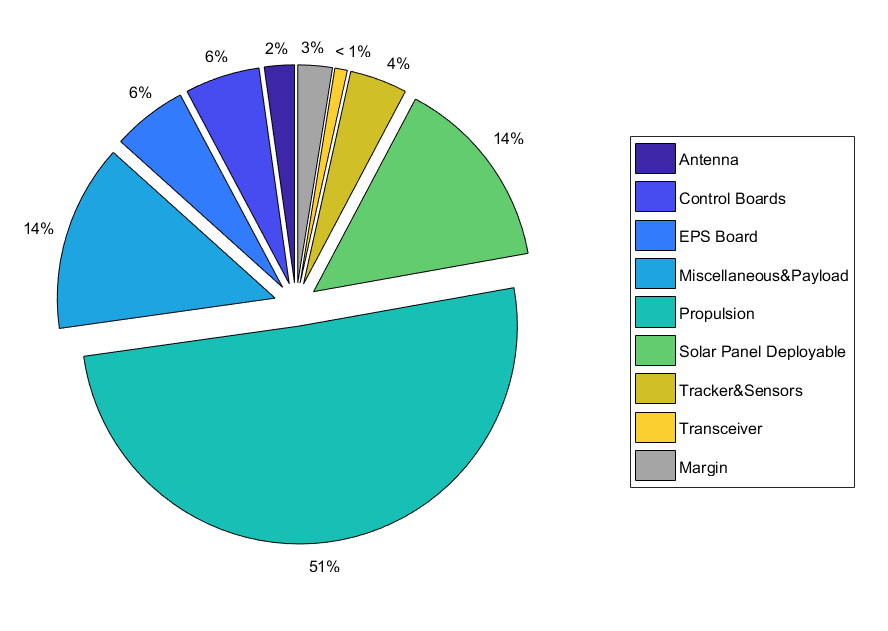
\includegraphics[width=0.90\textwidth]{volume}
											\caption{Volumenbudget für das angenommene Design}
											\label{fig:volume}
										\end{figure}
								
						\subsubsection{Leistungsbudget}
Das Leistungsbudget \abb{fig:power} gibt einen Überblick über den Verbrauch der verschiedenen Komponenten. Es gibt die Entladung der Batterie auf der Schattenseite der Erde wieder (Req. Battery Power) und wie in den anderen Budgets die Spanne zur Systemuntauglichkeit (Margin). Der Antrieb nimmt mit 32 \% insgesamt den größten Anteil des Energieverbrauchs ein.
				
										\begin{figure}[!h]
											\centering
												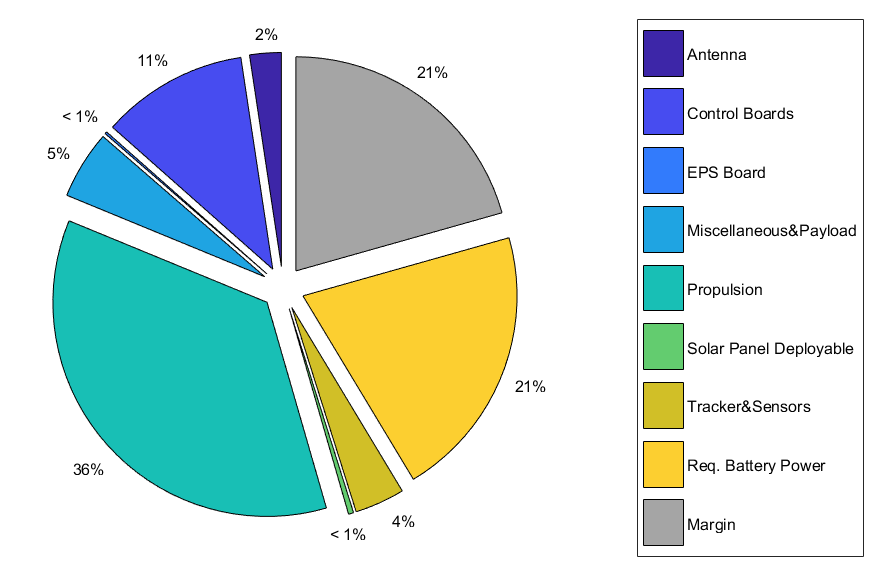
\includegraphics[width=0.90\textwidth]{power}
											\caption{Energiebudget für das angenommene Design}
											\label{fig:power}
										\end{figure}
Um das Leistungsbudget zu erstellen muss die Höhe der Umlaufbahn und der Orbit $\beta$ Winkel angegeben werden \abb{fig:power1}. diese wurden mit 1150 m und 0 \textdegree{} angenommen \tab:{cubesatdesign}.
\begin{figure}[!h]
	\centering
		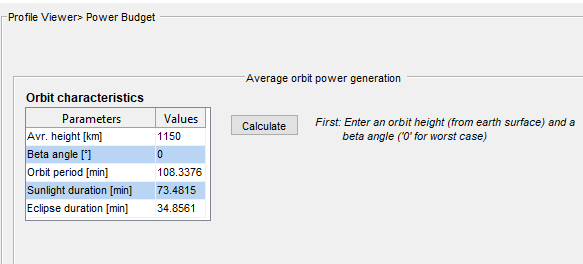
\includegraphics[width=0.70\textwidth]{graphics/power1.png}
	\caption{QuSAD: Orbit Charakteristik Eingabewerte}
	\label{fig:power1}
\end{figure}
Mit den eingegebenen Werten werden automatisch weitere Größen berechnet. Nach der Zuordnung der verschiedenen Solarpanele an die vorgesehene Position des CubeSats und der Eingabe der maximalen Missionsdauer (\abb{fig:power2})kann die Energieerzeugung während einer Erdumrundung kalkuliert werden (\abb{fig:power3} und \abb{fig:power4}).										

		 \begin{figure}[!h]
				\centering
					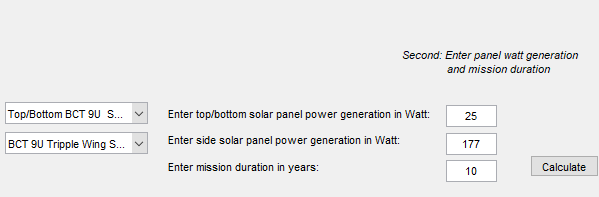
\includegraphics[width=0.70\textwidth]{graphics/power2.PNG}
				\caption{QuSAD: Auswahl der Solarpanele und der Missionsdauer}
				\label{fig:power2}
			\end{figure}
			
			\begin{figure}[!h]
				\centering
					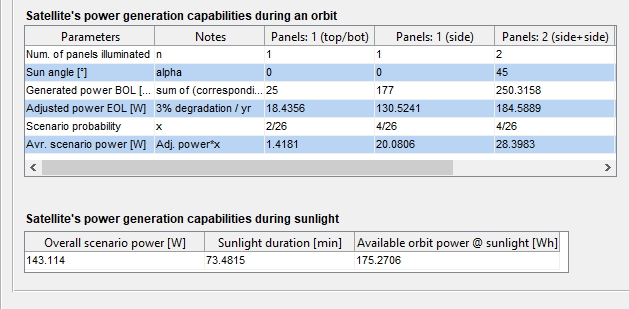
\includegraphics[width=0.70\textwidth]{graphics/power3.png}
				\caption{QuSAD: Energieerzeugung pro Orbit 1}
				\label{fig:power3}
			\end{figure}
			
			\begin{figure}[!h]
				\centering
					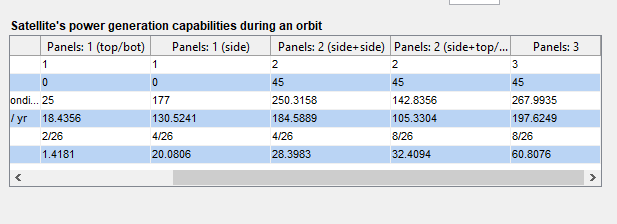
\includegraphics[width=0.70\textwidth]{graphics/power4.PNG}
				\caption{QuSAD: Energieerzeugung pro Orbit 2}
				\label{fig:power4}
			\end{figure}
Da das Haupttriebwerk und das RCS-System nicht dauerhaft betrieben werden, muss für diese Komponenten eine Prozentuale Brenndauer angegeben werden. Die mit den getroffenen Annahmen über die Brenndauer veränderten Werte  \tab:{cubesatdesign} können manuell geändert werden. Der Energieverbrauch der einzelnen Komponenten pro Orbit wird direkt angezeigt (\abb{fig:power5}). 
			
			\begin{figure}[!h]
				\centering
					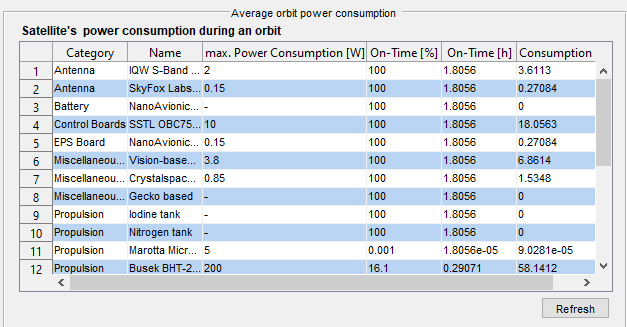
\includegraphics[width=0.70\textwidth]{graphics/power5.png}
				\caption{QuSAD: Energieverbrauch pro Orbit}
				\label{fig:power5}
			\end{figure}
Die von QuSAD angenommenen Werte zur bestimmung des Energieüberschusses sind in  \abb{fig:power6} zusammengefasst. 
			
			\begin{figure}[!h]
				\centering
					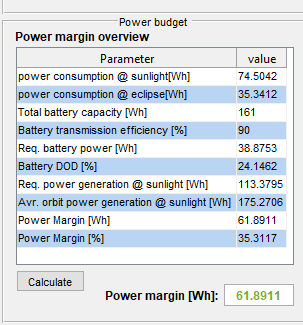
\includegraphics[width=0.70\textwidth]{graphics/power6.png}
				\caption{QuSAD: Überblick Energieüberschuss}
				\label{fig:power6}
			\end{figure}
Zur Berechnung des Budgets wird eine Batterieeffizienz von 90 \% angenommen. Außerdem wird mit einer Verschlechterung der Energieerzeugung von 3 \% pro Missionsjahr gerechnet. Der Wert “Power margin” gibt den Energieüberschuss eines Orbits in Wh an (\abb{fig:power6}). Das Budget in \abb{fig:power} stellt den Zustand des CubeSats nach der angegebenen Missionsdauer in \abb{power2} dar. Die Energieproduktion pro Orbit sinkt mit dem Fortlaufen der  Mission. Somit ist der Energieüberschuss bei Missionsstart deutlich höher. 			
			
			
			\section{Auswertung und Optimierung des Designs}

				
